\begin{figure}[t]
  \centering
  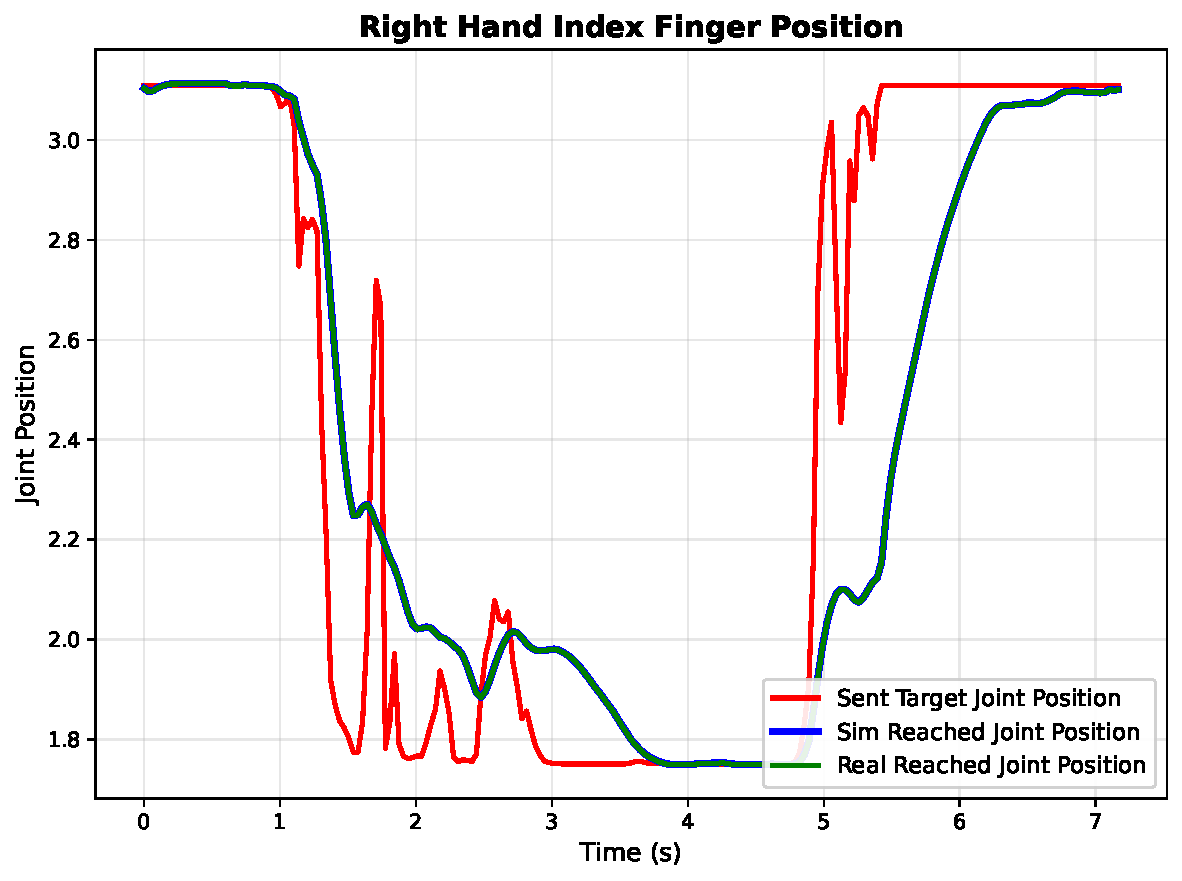
\includegraphics[width=0.9\linewidth]{figures/hybrid-control_pic.pdf}
  \caption{ \textbf{The comparison of sent target joint position and the actual reached joint position in both simulation and real-world.} The red, blue, and green curves exhibit similar overall trends. Compared with the blue and green curves, the red curve shows a deviation in joint position at the same time step, while the blue and green traces overlaps throughout. This discrepancy points to the gap between the simulated and real-world dynamics, and adopting the hybrid control keeping the dynamics consistency between the simulation and the real robot.}
  \label{fig:hybrid-control}
\end{figure}